\section{ANTELOPE (Semi-supervised)}
\label{subsec:unsupervised}

The semi-supervised machine learning approach broadens the discovery potential of the search through the use of data-driven training, where no signal model is provided.
While broad sensitivity is a general goal of LHC searches, it is particularly motivated in the case of dark QCD models, which can lead to widely varying topologies depending on the values of model parameters.

%--------------------
\subsection{Architecture Fundamentals}
The model-independent search region of this analysis is implemented with a novel ML approach that builds on the PFN architecture to construct a tool that is capable of performing low-level anomaly detection with permutation-invariant inputs.
This tool, referred to as \textbf{ANomaly deTEction on particLe flOw latent sPacE (ANTELOPE)}, is a custom solution designed for this analysis.

Figure~\ref{fig:antelope_arch} provides a diagram of the ANTELOPE architecture. ANTELOPE uses the trained PFN network described in the previous section to generate a permutation invariant event representation $\mathcal{O}$ from track level inputs. The $\mathcal{O}$ basis is used as the input for a \textit{variational autoencoder} (VAE). A VAE is a common variation of a standard AE; the AE becomes \textit{variational} if the latent space is constructed through Gaussian sampling rather than a vector of weights, as described further in Ref.~\cite{vae2}. VAEs have been used in previous ATLAS searches to model low-level particle information, such as the search presented in Ref.~\cite{yxh} which used the recurrent architecture described in Ref.~\cite{vrnn}. One of the limitations of a recurrent architecture is the need to order the low-level inputs, which affects the performance of the tool. Jet track information is intrinsically unordered, and therefore a permutation invariant approach removes this element of arbitrary decision making from the modeling process. 

\begin{figure}[!htbp]
\centering
   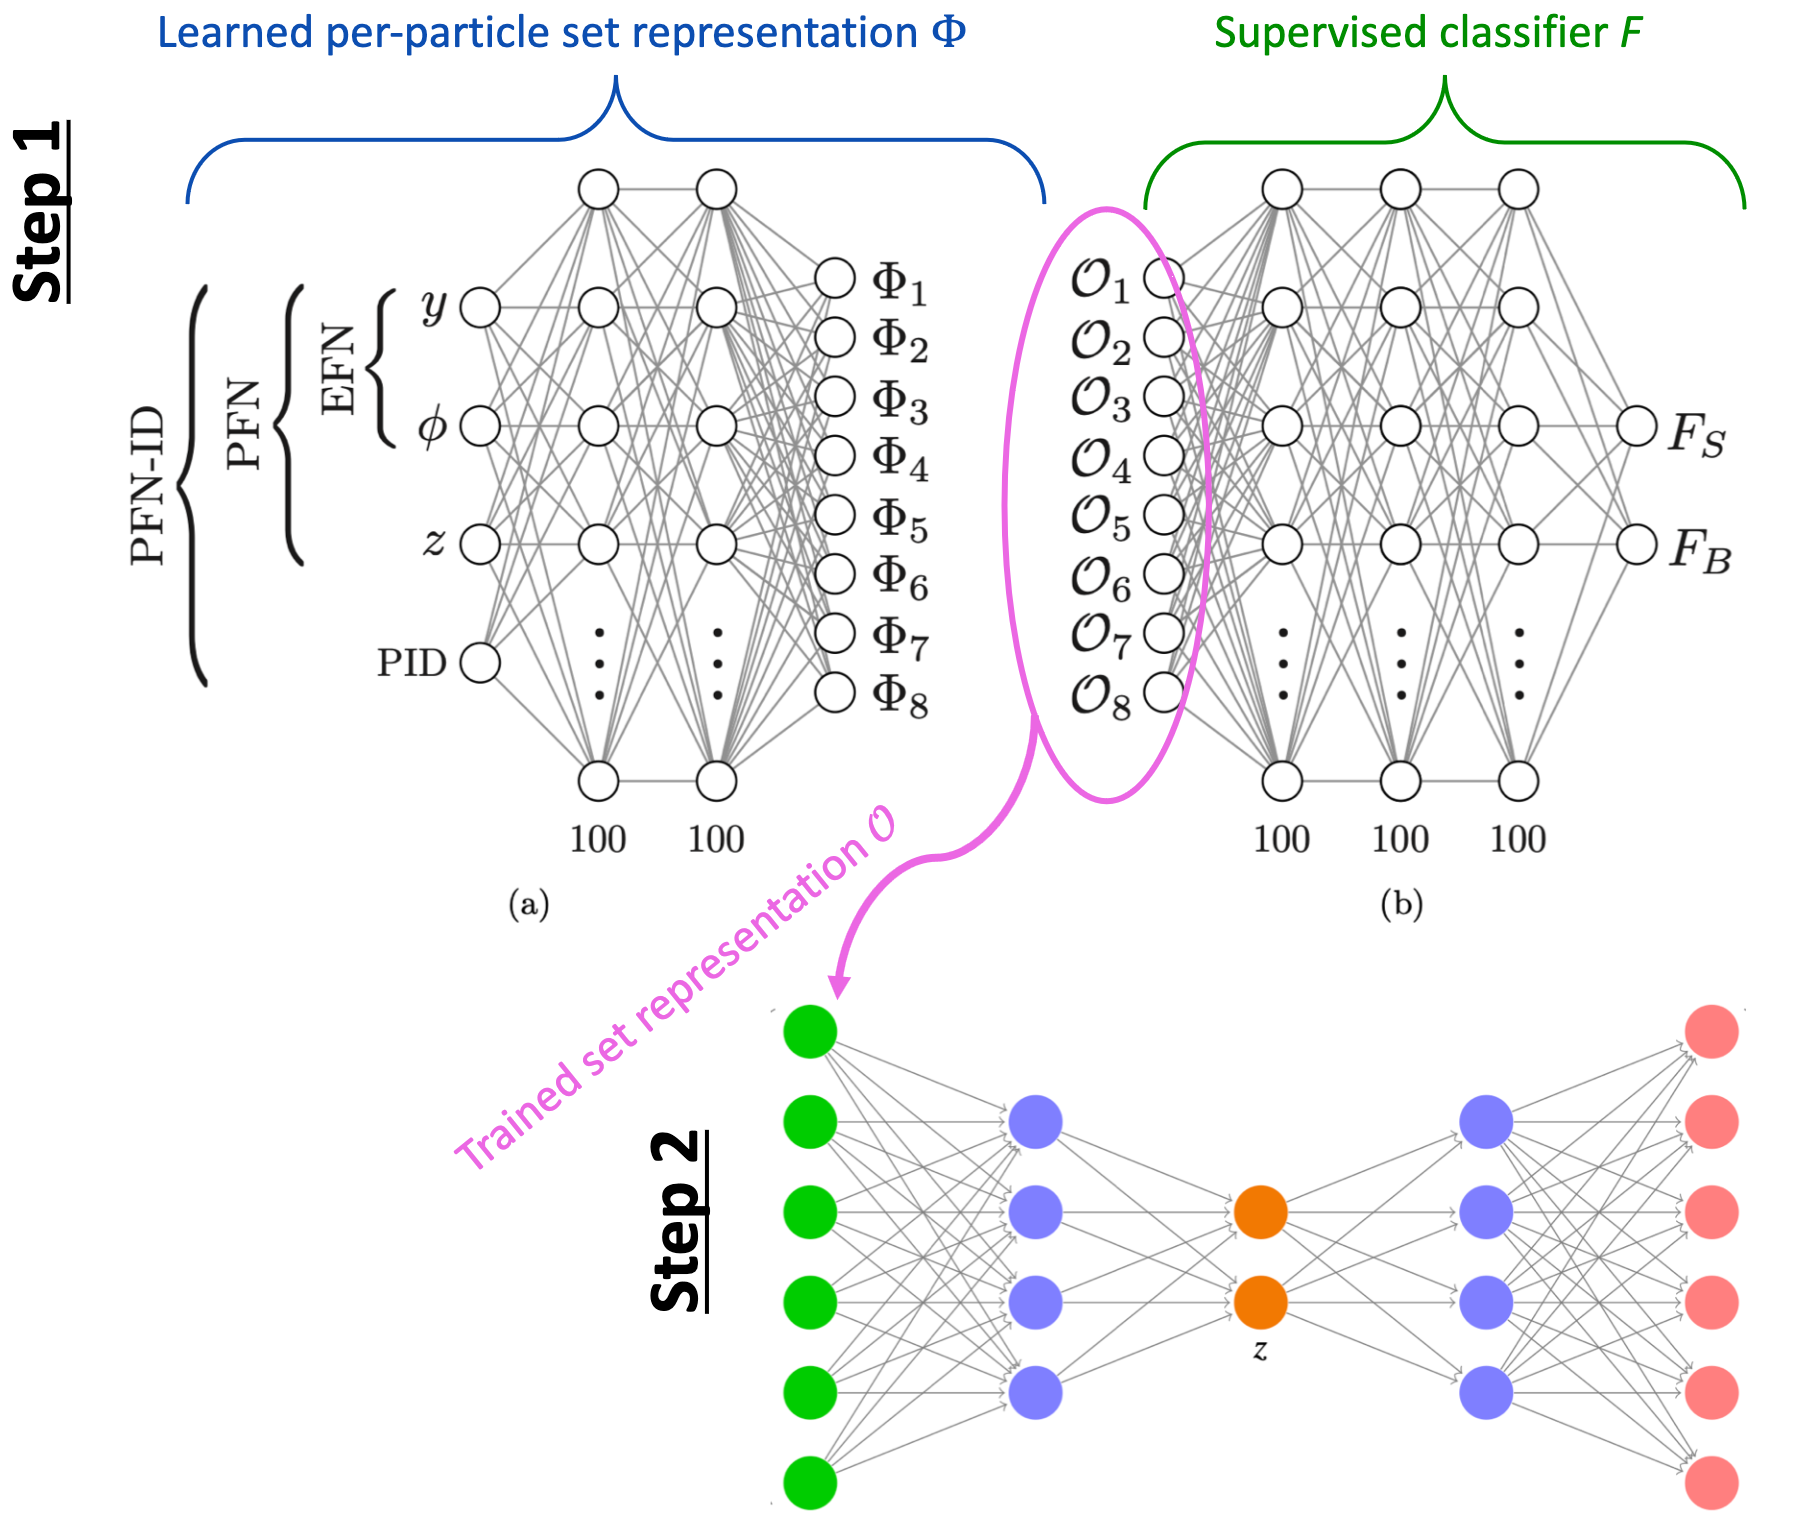
\includegraphics[width=0.9\textwidth]{figures/ml/antelope_arch}
    \caption{An annotated diagram of the ANTELOPE architecture. Step 1 illustrates the PFN which is fully trained before its use in the ANTELOPE network. Step 2 illustrates the variational auto-encoder. The Gaussian sampling of the latent space is shown, illustrating how the VAE differs from the AE shown in Figure~\ref{fig:ae}. 
    \label{fig:antelope_arch}}
\end{figure}

The input to ANTELOPE architecture is the same 6 track variables for the leading two jets, as presented in Section~\ref{sec:input_model}. The track information is encoded to the PFN $\mathcal{O}$ event representation using the pre-trained $\Phi$ neural network (trained according to the steps outline in Section~\ref{sec:pfn_training}). The VAE is then trained in an \textit{unsupervised} way using inputs encoded to $\mathcal{O}$ from data events only. Here \textit{unsupervised} means that the VAE is given no knowledge of the signal model during training. There is implicit knowledge of the signal model in the $\mathcal{O}$ encoding, so the full ANTELOPE network is considered semi-supervised, while the VAE component is unsupervised. A visual example of the $\mathcal{O}$ input to the VAE portion of the ANTELOPE is given in Figure~\ref{fig:antelope_input_rep}. 

\begin{figure}[!htbp]
\centering
   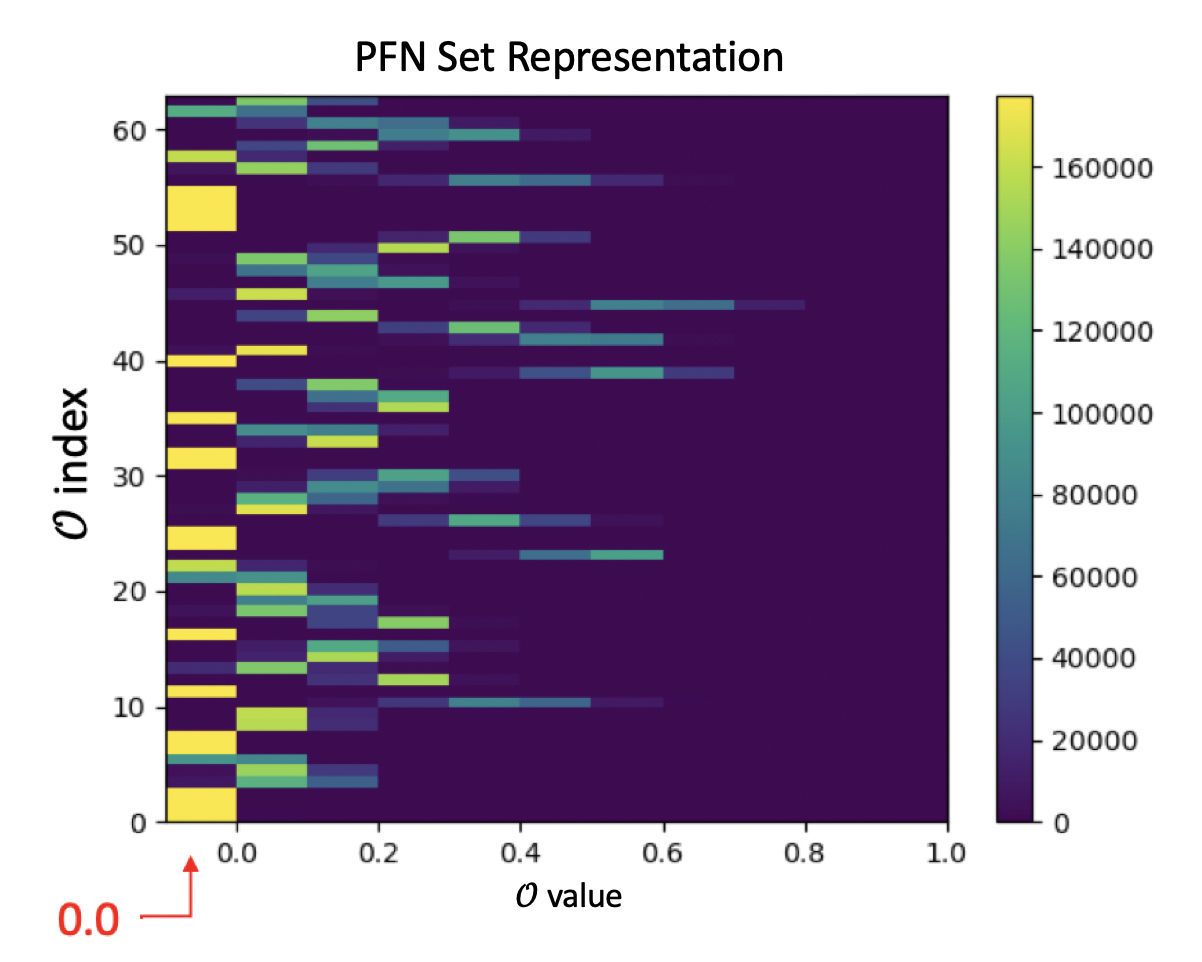
\includegraphics[width=0.7\textwidth]{figures/ml/antelope_input_rep}
    \caption{A visual representation of the 64 PFN $\mathcal{O}$ which create the input for the VAE component of ANTELOPE. The plot is 2D histogram of the PFN $\mathcal{O}$ index (0-63) versus the value assumed by that index. Many entries have a $\mathcal{O}$ value of exactly 0.0. To visually separate these from entries with a small but non-zero $\mathcal{O}$ value, any entries with value = 0.0 are moved to value = -0.01 (leftmost column) for the purpose of the plot only.
    \label{fig:antelope_input_rep}}
\end{figure}

The VAE is trained to minimize the reconstruction error, or the difference between its input and output layer. This pushes it to uncover patterns in the data, which is predominantly composed of SM processes. Any rare events in the data which present patterns inconsistent with the majority of the data will receive a higher reconstruction error. This error is used to create the anomaly score. 

%--------------------
\subsection{Training}

The VAE stage of the ANTELOPE network is trained over 500k data events.
The input dimensionality of the VAE has to match the encoded $\Phi$ dimension of the PFN, in this case 64. 
The encoding portion of the VAE has a hidden layer with 32 nodes,  and a latent space dimension of 12.
The decoding portion has another hidden layer of 32 nodes, and the output layer has a dimension of 64 to match the input layer.
All layers use a \textsc{relu} activation~\cite{scikit-learn} except for the output layer which uses a \textsc{sigmoid} activation~\cite{scikit-learn}, to restrict the output between 0 and 1.
As in the PFN, the Adam optimizer~\cite{adam}~\cite{scikit-learn} is used.

The network is trained for 50 epochs, with a learning rate of 0.00001. 
The VAE was observed to need a very small learning rate to effectively minimize the loss.
The loss $\mathcal{L}$ is the sum of two terms, the mean-squared error (MSE) of input-output reconstruction, and the Kullback-Leibler divergence (KLD).

\begin{equation}
\label{eq:vrnnloss}
\mathcal{L} = \sum_i L_i = \sum_i | \Phi_i^2 - \Phi\prime_i |^2 + \lambda D_{\text{KL}}
\end{equation}

Figure~\ref{fig:antelope_loss} shows the loss during training.
The validation events are seen to have a lower loss than the training events, indicating there is no issue with overtraining.
\begin{figure}[!htbp]
\centering
   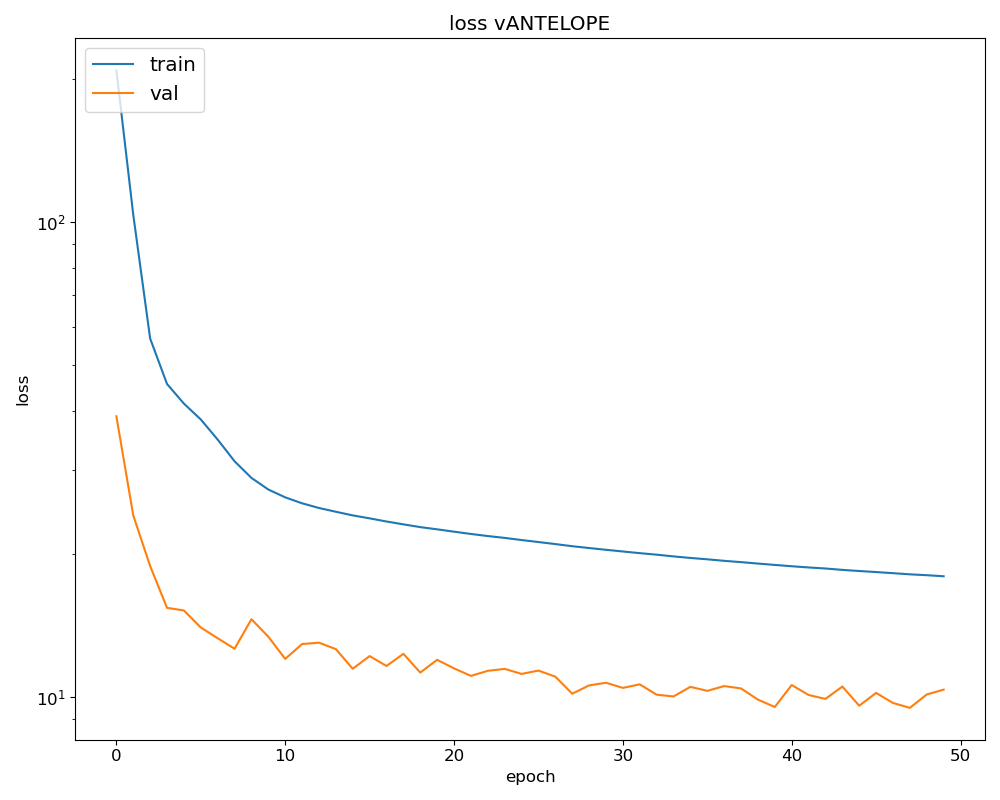
\includegraphics[width=0.5\textwidth]{figures/ml/antelope_loss}    
    \caption{ANTELOPE architecture loss during training as a function of epoch.
    \label{fig:antelope_loss}}
\end{figure}


%--------------------
\subsection{Performance}
\label{subsec:antelope_perf}

As with the PFN, the ANTELOPE performance is assessed via the ROC and AUC. 
Figure~\ref{fig:antelope_score} shows the anomaly score and an example ROC curve.
The anomaly score is calculated from the loss as defined in \ref{eq:vrnnloss}.
The score is produced by applying a sigmoid function to the loss to restrict its output between 0.0 and 1.0:

\begin{equation}
\label{eq:asfunc}
a = \frac{1}{1+e^{-\mathcal{L}}}
\end{equation}
where $a$ is the anomaly score and $\mathcal{L}$ is the VAE loss. Because the loss is always positive, the sigmoid transformation effectively restricts the anomaly score range between 0.5 and 1.0. The anomaly score is observed to range between 0.6 and 1.0, as the reconstruction loss is always non-zero. Following a similar sensitivity optimization as presented for the PFN score selection in Section~\ref{sec:pfn_performance}, a selection of \textbf{anomaly score > 0.7} is chosen for use in the analysis.

\begin{figure}[!htbp]
\centering
   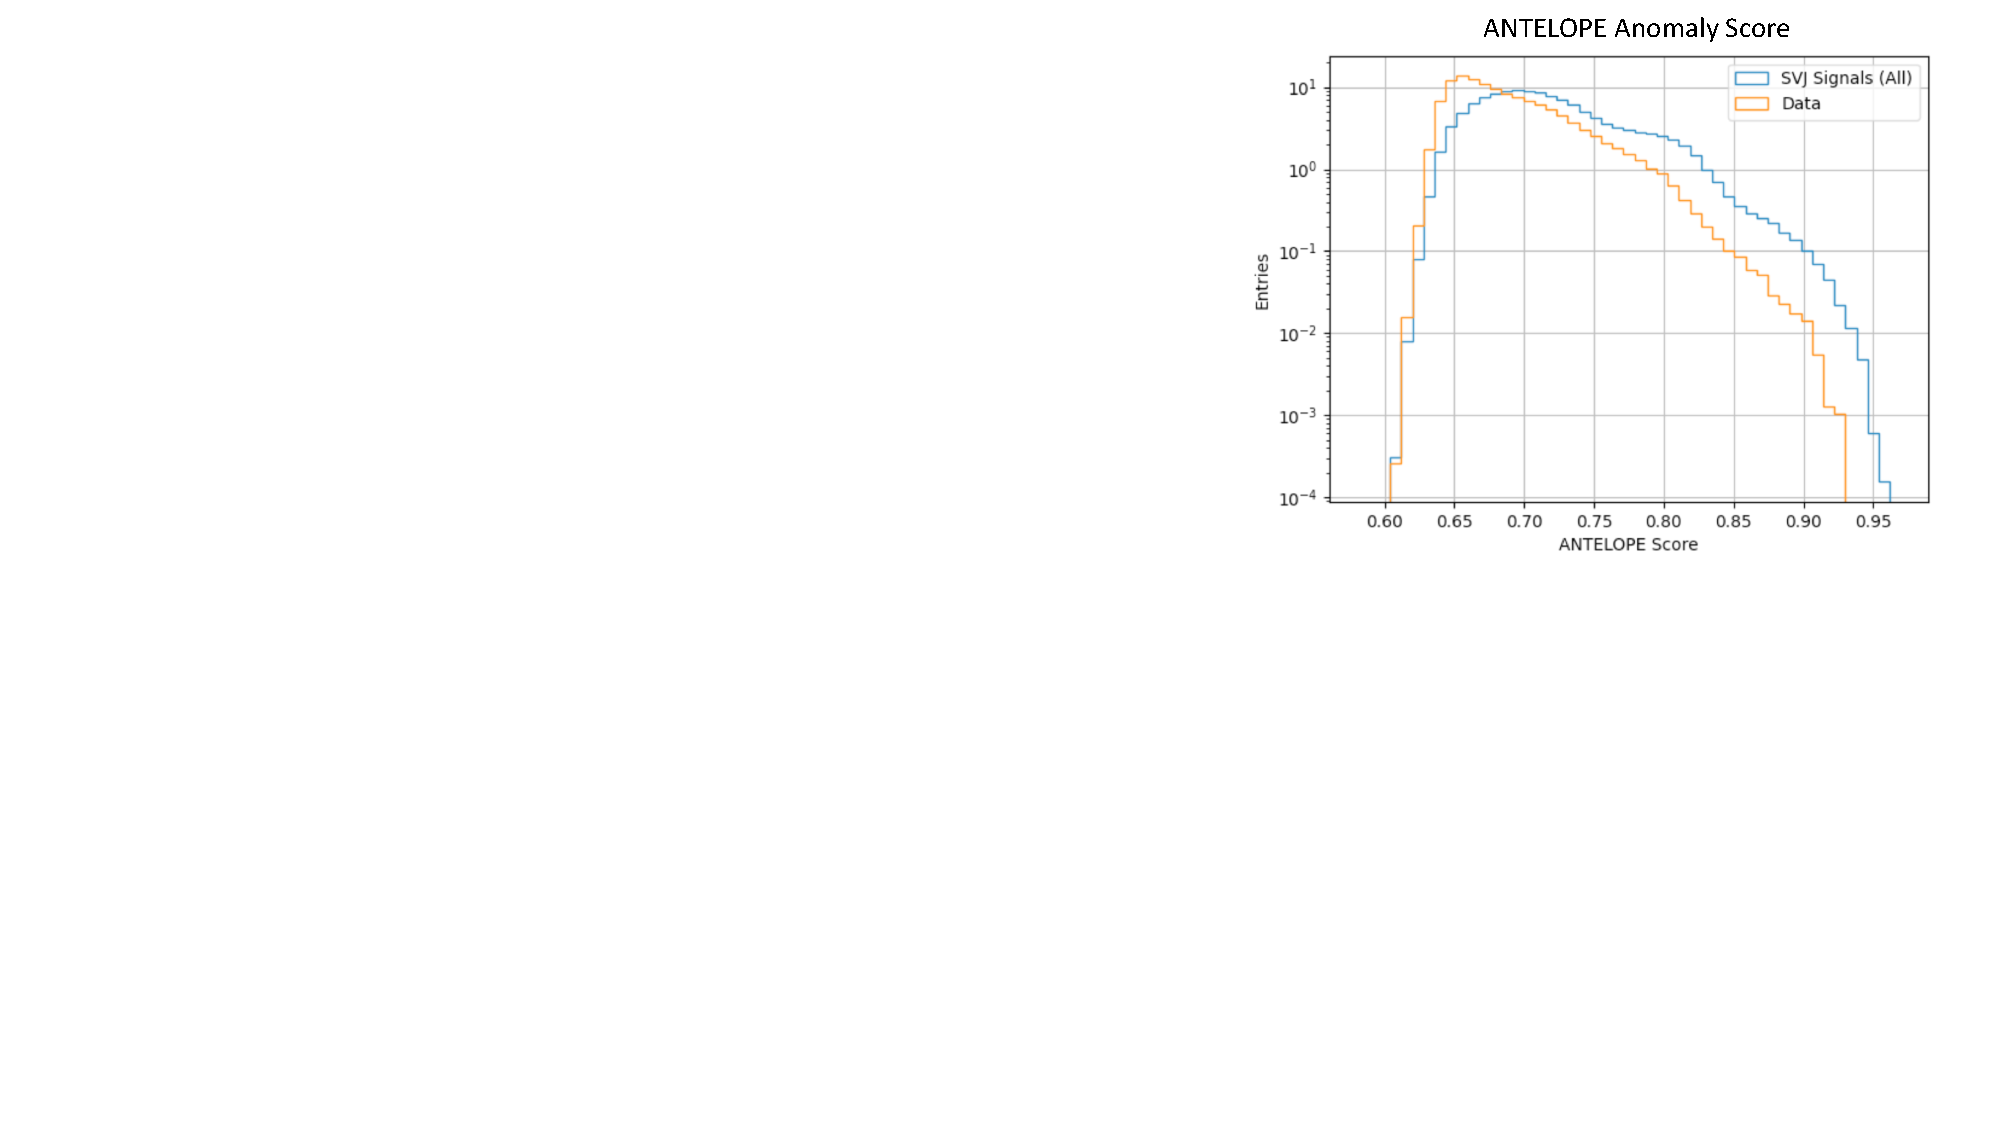
\includegraphics[width=0.48\textwidth]{figures/ml/antelope_score.pdf}
   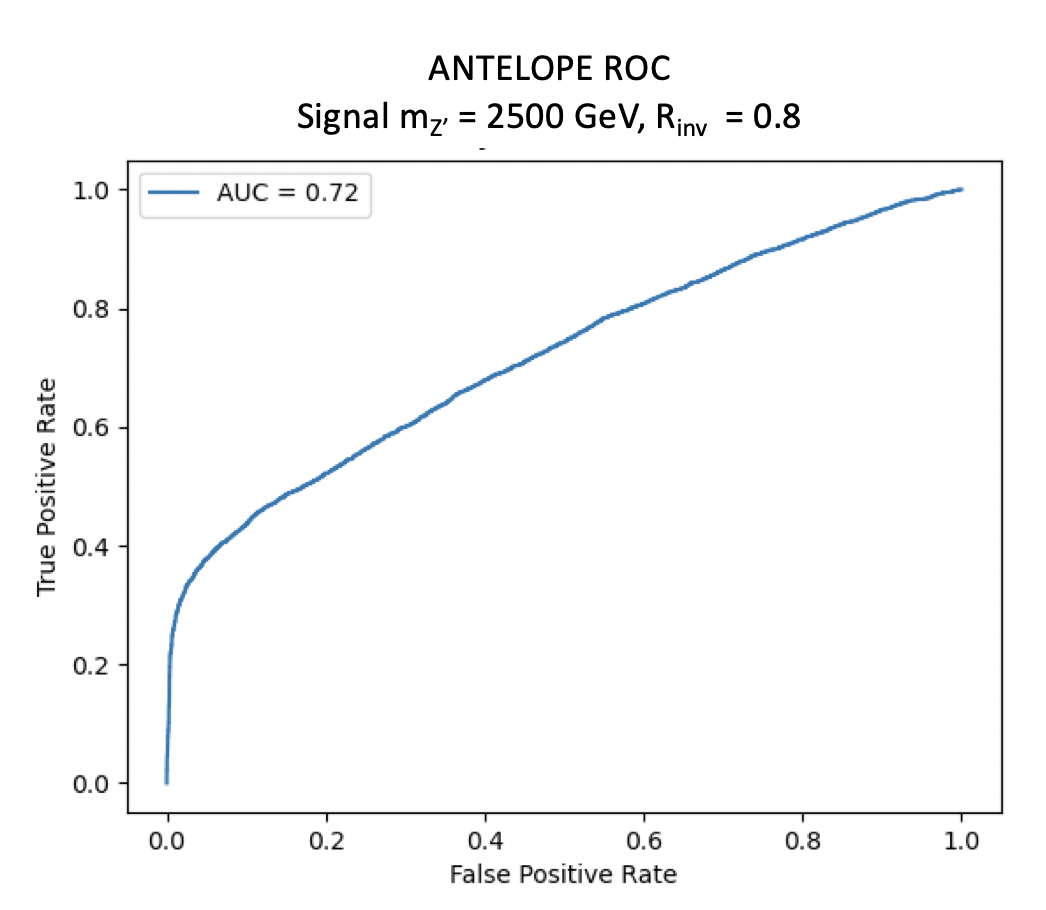
\includegraphics[width=0.48\textwidth]{figures/ml/antelope_roc}
    \caption{Anomaly score distribution (left), comparing all data (orange) and all SVJ signals (blue). The signals have a small but consistently higher score than the data, indicating that they are tagged as more anomalous by ANTELOPE. A ROC curve for an example signal point is also shown (right).
    \label{fig:antelope_score}}
\end{figure}

Figure~\ref{fig:antelope_AUC_score_grid} shows the AUC of the ANTELOPE across the SVJ signal grid, demonstrating discrimination capability across varying SVJ signal models.
Compared to the supervised PFN method, the ANTELOPE is not as performant (as expected due to the absence of signal model in training).
However, the network is seen provide separation between signal and background for all signal points, as evidenced by AUC $> 0.5$ across the signal grid.

\begin{figure}[!htbp]
\centering
   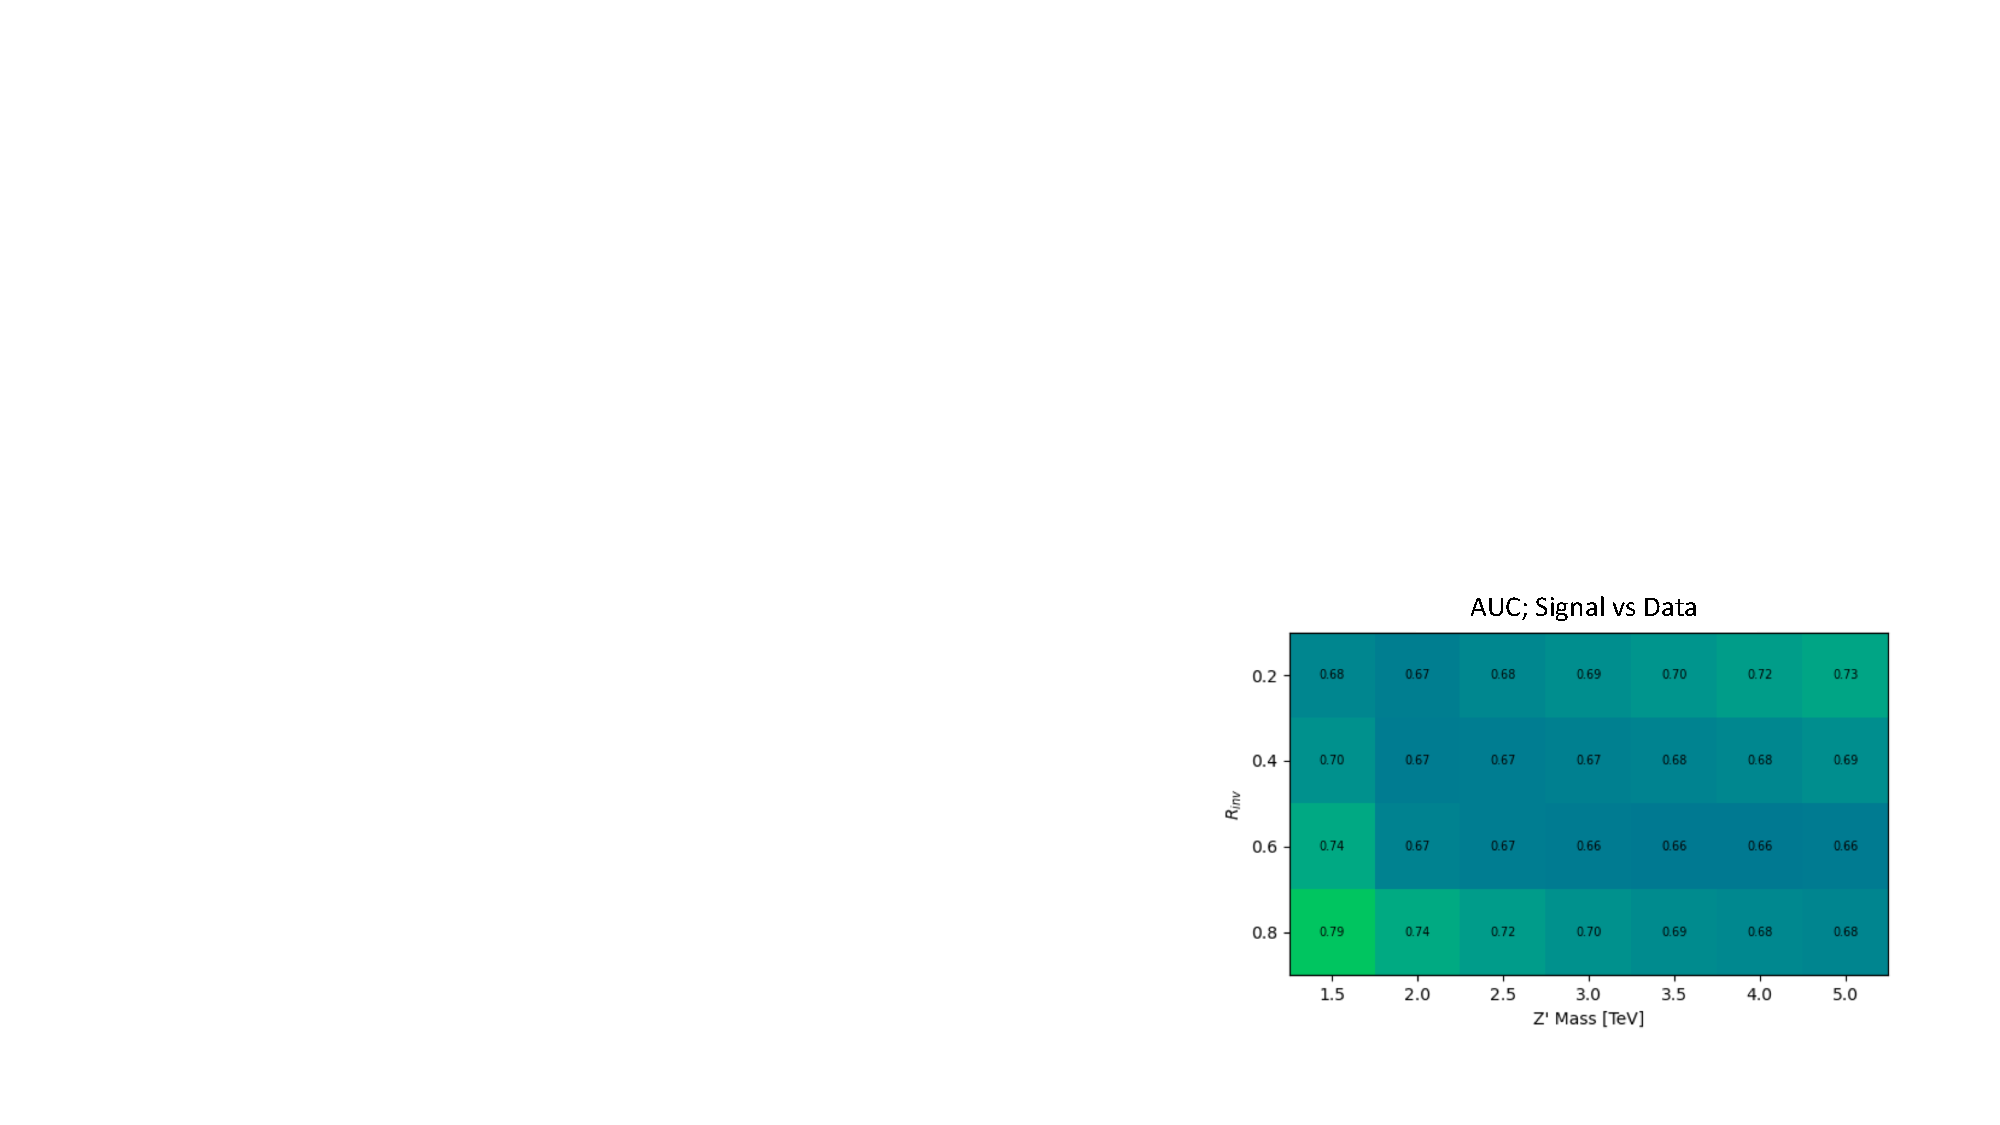
\includegraphics[width=0.7\textwidth]{figures/ml/antelope_AUC_score_grid}
    \caption{AUC from the ANTELOPE score for each signal in the SVJ grid.
    \label{fig:antelope_AUC_score_grid}}
\end{figure}

\paragraph{Model Independence} 

The unsupervised component of training the ANTELOPE network is expected to give it a more generalized sensitivity to new physics with \met~and jet activity, beyond the scope of the SVJ grid. 
To assess this, alternative signal models are evaluated with the trained ANTELOPE network.

The following alternate signal models were considered: 
\begin{itemize}
\item Z' $\rightarrow$ $t\bar{t}$ 
\item W' $\rightarrow$ WZ 
\item Gluino pair production $\rightarrow$ R-hadron + LSP (\met) with gluino masses 2000/3000 GeV, LSP mass 100 GeV, and lifetime 0.03 ns (LSP = \textit{lightest supersymmetric particle})
\item Emerging jets s-channel with mass 1000 GeV and lifetime 1ns 
\end{itemize}

Figure~\ref{fig:antelope_altsig} shows the distribution of these signals in the PFN score and the ANTELOPE anomaly score.
The benefit of the ANTELOPE in enhancing model independence is clearly seen through the boost in performance for certain non-SVJ signal models.
The gluino and emerging jet signals in particular are marked as highly anomalous by the ANTELOPE, but are marked as evenly background-like and signal-like by the PFN.
This observation demonstrates that the use of the ANTELOPE network in this analysis has the potential to expand our sensitivity to include alternate signal models that could be marked as highly anomalous with the anomaly score.

\begin{figure}[!htbp]
\centering
   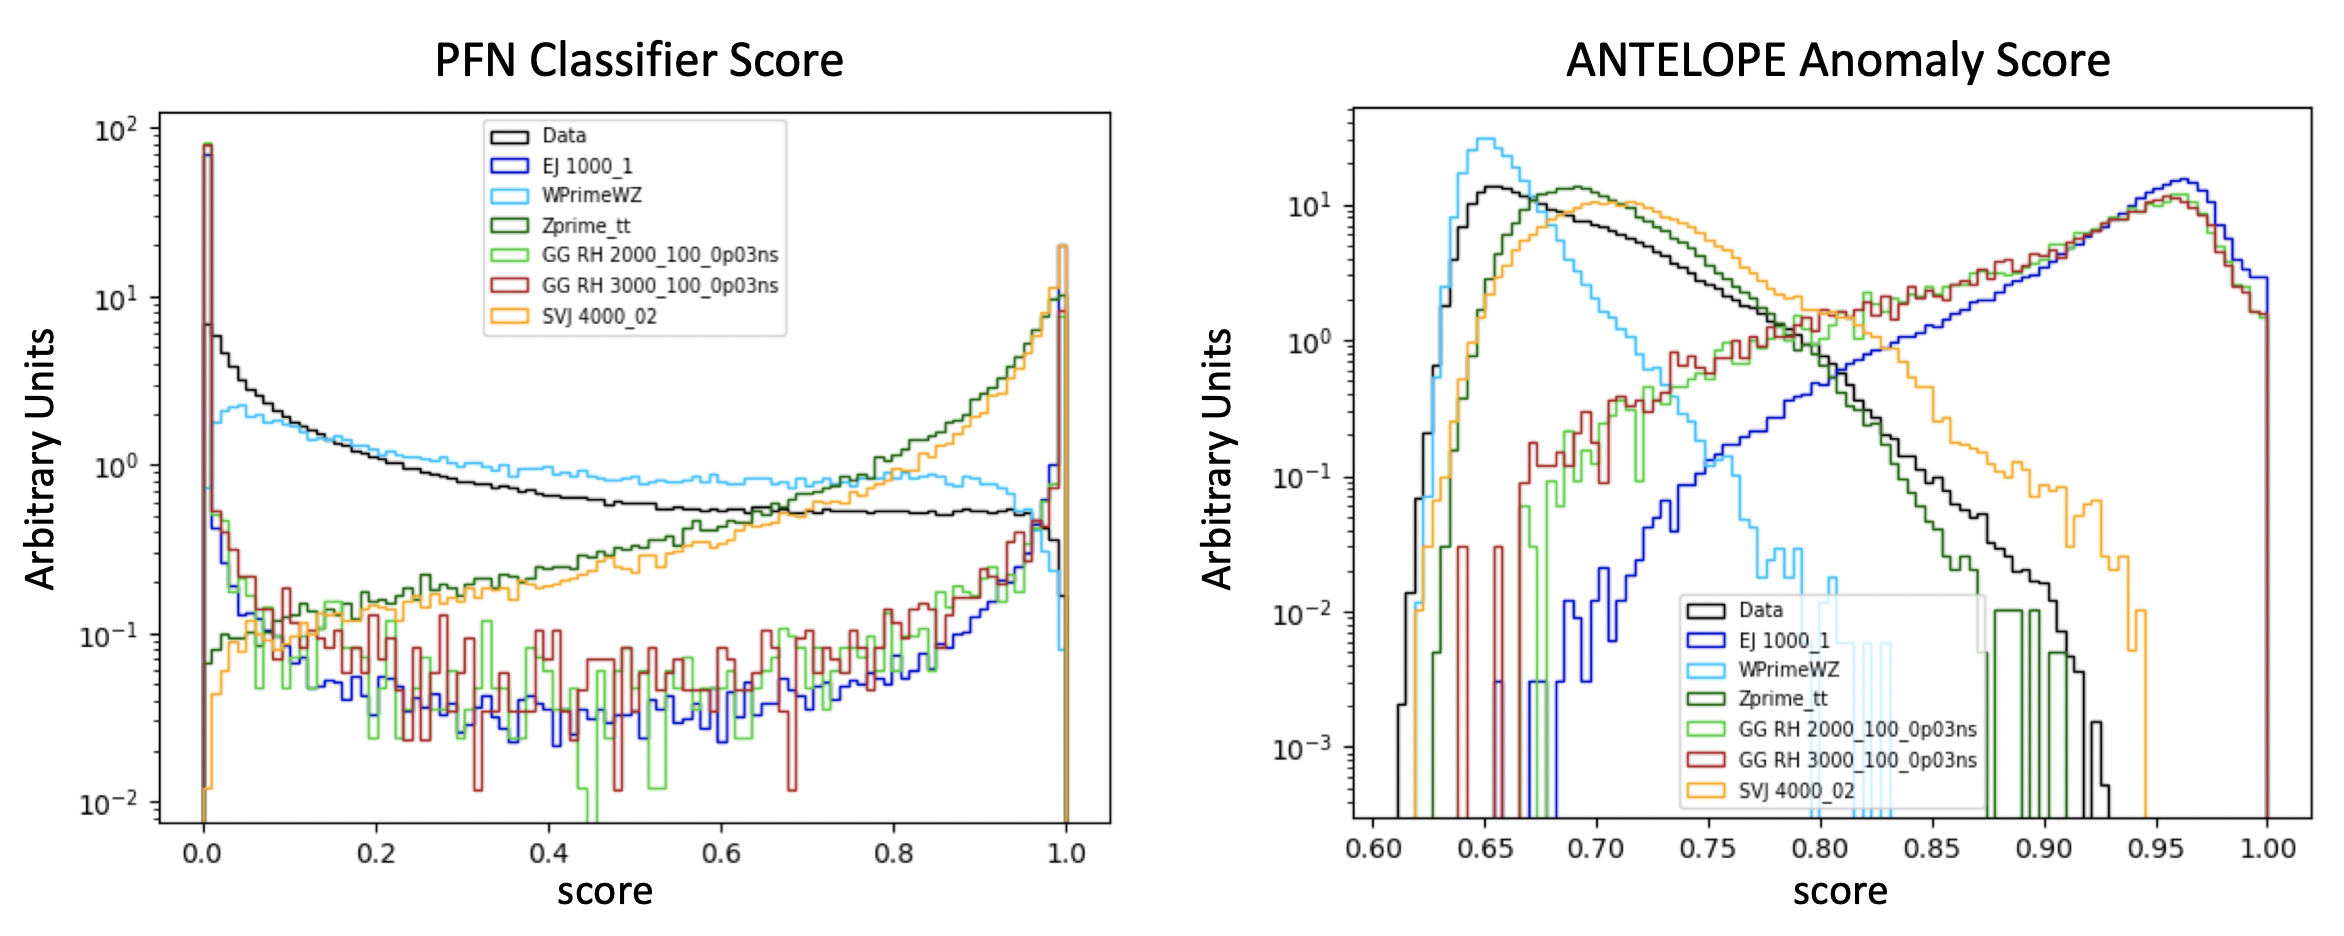
\includegraphics[width=0.98\textwidth]{figures/ml/antelope_vs_pfn_score}
    \caption{Comparing data and the alternate signal models for the PFN score (left) and ANTELOPE score (right). The emerging jet signal (dark blue) and gluino R-hadron signals (red, light green) are an example of the advantage of the model-independent ANTELOPE approach. These signals have a bimodal shape in PFN score but are clearly tagged with a high anomaly score by the ANTELOPE.
    \label{fig:antelope_altsig}}
\end{figure}





